\documentclass[titlepage]{article}

\usepackage[margin=1in]{geometry}
% some more shit for the title
\usepackage[T1]{fontenc}
\usepackage{babel}

% Tables and stopping them from displaying in a different section
\usepackage{booktabs}
\usepackage[section]{placeins}

% for inserting images into the document, setting file path, and allowing rotation of inserted images 
\usepackage{graphicx}
\graphicspath{ {./images/} }
\usepackage{rotating}
\usepackage[table]{xcolor}
% mostly just for putting text in math equations
\usepackage{amsmath}
% for aligning the text to the left
\usepackage[document]{ragged2e}

% for inserting hyperlinks in the document, use \url{url} or \href{url}{text}
\usepackage{hyperref}
\usepackage{calligra}
\usepackage[T1]{fontenc}
\usepackage{siunitx}
\usepackage{caption}
\usepackage{multirow}
\usepackage[export]{adjustbox}
\usepackage{tikz}
\usepackage{pgfplots}
\pgfplotsset{soldot/.style={color=black,only marks,mark=*},
	             holdot/.style={color=black,fill=white,only marks,mark=*},
		                  compat=1.12}

\begin{document}
\title{\textbf{Lab 2: Electric Field and Potential}}
\author{
    Zachary Pouska\\
    \texttt{001103193}\\
    \and
    Natalie Tran \\ 
    \texttt{000698629}\\ \\
} 

\date{PHYS 236 | Fall 2022\\
Date performed: 09/21/2022}


	\maketitle



	\section{Purpose}
	To study the relationship between electric field and the electric potential difference associated with it.
	\section{Theory}	
	The relationship between the electric field and electric potential difference will follow the equation \(\Delta V = -\int_{a}^{b} \vec{E} \cdot ds\), which simplified is \(\Delta V = \frac{k_{e}q}{r}\). This means electric potential will have a opposite yet linear relationship with the electric field, while having an inverse relationship with distance.
	\section{Experiment Analysis}
    
    Using the following equations, we were able to predict many of the results we found during this lab:
    $$\Delta V = -\int_a^b \vec{E}\cdot d\vec{s} $$
    $$V= k_e \int_a^b \frac{dq}{r} $$




	\section{Procedure}
    The experiment is begun by "drawing" the patterns used for the experiments on the conductive surface using conductive ink. This step was performed by our instructor beforehand. 
    \subsection{Perimeter of Conductive Ink and Point Charge}
    The configuration of electrodes below was used for this first part of the experiment. The small circular electrode (white dot) at the center was held at 10 Volts. The green dots indicate where the voltages were measured. 7 points were taking from each side of the positive electrode.

    \FloatBarrier
    \begin{figure}[hbt!]
        \centering
        \caption{Perimeter of conductive ink and point charge setup}
        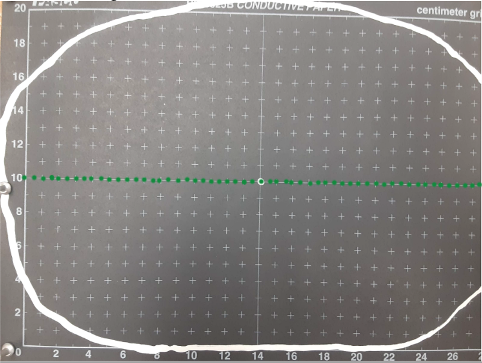
\includegraphics[scale=0.8]{procedure/part1}
    \end{figure} 
    \FloatBarrier



    

    \subsection{Two Point Charges}
    The goal of this experiment was to determine the shape of the equipotential lines resulting from two point charges on a conductive surface. In order to find these equipotential lines, we probed the conductive plate with a digital multimeter, and recorded the results on a piece of graph paper. We measured only four equipotential lines between the two point charges, ranging between 6V and 1.5V. In order to determine the electric field, we use an equation to estimate the magnitude from a potential difference between two points $a$ and $b$.
    $$E=\frac{-V_b-V_a}{\Delta x}$$



    \subsection{Two Plate Capacitor}
    This experiment was similar in nature to the previous one, but just with a different setup. We connected our power supply to the two electrodes of the "capacitor," and begun measuring our equipotential lines. We unfortunately only measured two whole lines, as the setup we received for the lab had the two electrodes very close together. The following is an example of a setup for this lab: 

    \FloatBarrier
    \begin{figure}[hbt!]
        \centering
        \caption{Two Plate Capacitor Setup}
        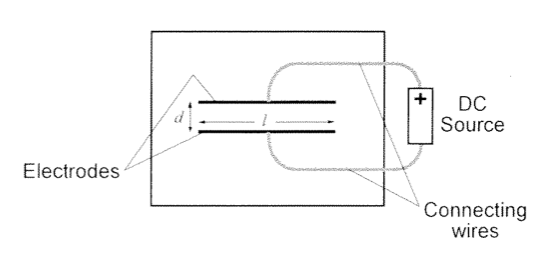
\includegraphics[scale=0.4]{procedure/capacitor}
    \end{figure} 
    \FloatBarrier


    \subsection{One Point and One Line}
    Again, this lab follows a similar set of steps to the previous two. We being by connecting the point charge and line to the power supply leads, and beginning our measurement of the electric potentials. The following figure is another example of the setup for this experiment:

    \FloatBarrier
    \begin{figure}[hbt!]
        \centering
        \caption{Point and Line Example Setup}
        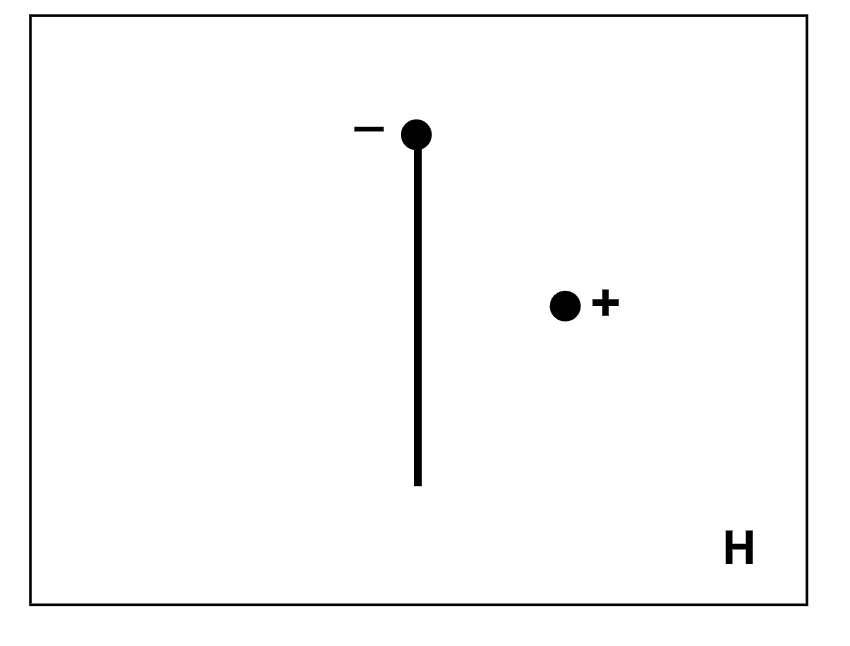
\includegraphics[scale=0.4]{procedure/pointline}
    \end{figure} 
    \FloatBarrier






	\section{Data and Graphs}
	\begin{center}
		\begin{minipage}[t]{0.4\textwidth}
		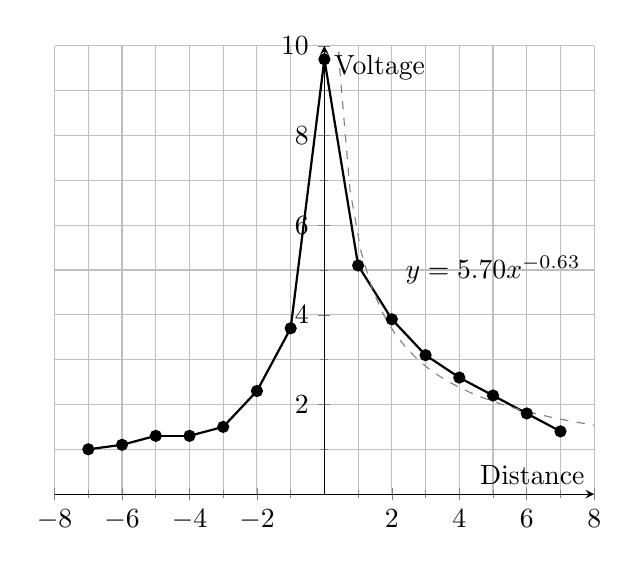
\begin{tikzpicture}
			\begin{axis}[grid=both,
				axis lines=middle,
				xmin=-8,xmax=8,
				ymin=0,ymax=10,
				xtick={-8,-6,-4,-2,0,2,4,6,8},
				ytick={2,4,6,8,10},
				minor tick={-7,-5,-3,-1,1,3,5,7,9},
				xlabel=Distance, ylabel=Voltage]

				\addplot[soldot] coordinates{(-7,1)(-6,1.1)(-5,1.3)(-4,1.3)(-3,1.5)(-2,2.3)(-1,3.7)(0,9.7)(1,5.1)(2,3.9)(3,3.1)(4,2.6)(5,2.2)(6,1.8)(7,1.4)};
			\draw[thick] (-7,1)--(-6,1.1);
			\draw[thick] (-6,1.1)--(-5,1.3);
			\draw[thick] (-5,1.3)--(-4,1.3);
			\draw[thick] (-4,1.3)--(-3,1.5);
			\draw[thick] (-3,1.5)--(-2,2.3);
			\draw[thick] (-2,2.3)--(-1,3.7);
			\draw[thick] (-1,3.7)--(0,9.7);
			\draw[thick] (0,9.7)--(1,5.1);
			\draw[thick] (1,5.1)--(2,3.9);
			\draw[thick] (2,3.9)--(3,3.1);
			\draw[thick] (3,3.1)--(4,2.6);
			\draw[thick] (4,2.6)--(5,2.2);
			\draw[thick] (5,2.2)--(6,1.8);
			\draw[thick] (6,1.8)--(7,1.4);
			\addplot[domain=0.1:8,dashed,gray] {5.7*x^(-0.63)};
			\node at (5,5) {$y = 5.70x^{-0.63}$};
			\end{axis}
		\end{tikzpicture}
		[Fig 1.1] Table 1.1 visualized in a graph.
		\end{minipage}
		\hspace{1cm}
		\begin{minipage}[t]{0.4\textwidth}
		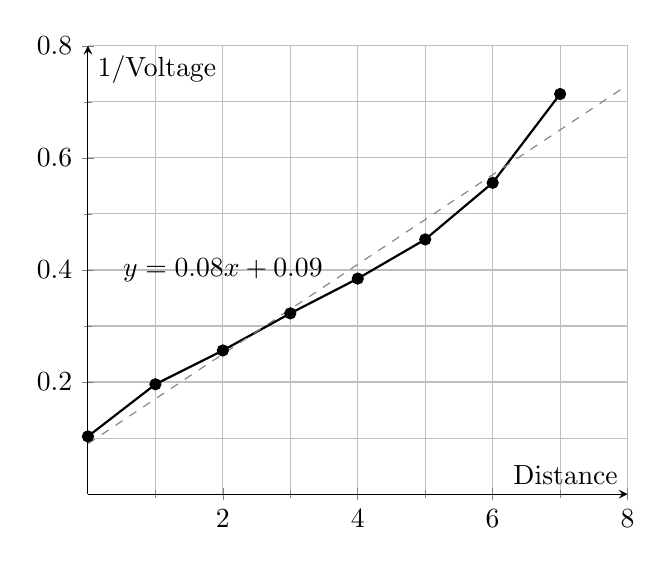
\begin{tikzpicture}
			\begin{axis}[grid=both,
				axis lines=middle,
				xmin=0,xmax=8,
				ymin=0,ymax=0.8,
				xtick={0,2,4,6,8},
				ytick={0,0.2,0.4,0.6,0.8},
				minor y tick num=1,
				minor x tick num=1,
				xlabel={Distance}, ylabel={1/Voltage}]

				\addplot[soldot] coordinates{(0,0.103)(1,0.196)(2,0.2564)(3,0.32258)(4,0.3846)(5,0.4545)(6,0.55555)(7,0.714)};
				\draw[thick] (0,0.103)--(1,0.196); 
				\draw[thick] (1,0.196)--(2,0.2564); 
				\draw[thick] (2,0.2564)--(3,0.32258); 
				\draw[thick] (3,0.32258)--(4,0.3846); 
				\draw[thick] (4,0.3846)--(5,0.4545); 
				\draw[thick] (5,0.4545)--(6,0.55555); 
				\draw[thick] (6,0.55555)--(7,0.714); 
				\addplot[domain=0:8,dashed,gray] {0.08*x+0.09};
				\node at (2,0.4) {$y = 0.08x+0.09$};
			\end{axis}
		\end{tikzpicture}
		[Fig 1.2] The linearization of Fig 1.1.
	\end{minipage}
	\end{center}
	\section{Results}
	\section{Questions}
	\section{Conclusion}
	
\end{document}
